\documentclass{report}
\usepackage{hyperref} % For clickable links and bookmarks
\usepackage{bookmark}

\usepackage[utf8]{inputenc}
\usepackage{enumitem}
\usepackage{amsmath} % For math environments
\usepackage{tcolorbox}
% ------------------------------
% Packages
% ------------------------------
\usepackage{graphicx}      % For including images
\usepackage{amsmath}       % Advanced math typesetting
\usepackage{amssymb}       % Math symbols (e.g., \mathbb, \leqslant, etc.)
\usepackage{amsthm}        % Theorem/lemma environments
\usepackage{stmaryrd}      % Extra math symbols (e.g., semantic brackets ⟦ ⟧)
\usepackage[short]{datetime} % Date formatting
\usepackage{caption}       % Custom captions for figures/tables
\usepackage{subcaption}    % Subfigures (side-by-side images)
\usepackage{multicol}      % Multi-column layout (e.g., notes, problems)
\setlength{\columnseprule}{1pt} % Vertical line between columns
\usepackage{soul}          % Highlighting (\hl{})
\sethlcolor{yellow}        % Highlight color
\usepackage[margin=1.75cm]{geometry} % Page margins

% ------------------------------
% Theorem Environments
% ------------------------------
\theoremstyle{definition} % Non-italic style for definitions/remarks
\newtheorem{remark}{Remark}
\newtheorem{theorem}{Theorem}
\newtheorem{lemma}{Lemma}
\newtheorem{definition}{Definition}
\newtheorem{corollary}{Corollary}
\newtheorem{property}[theorem]{Property}      % Shares counter with theorem
\newtheorem{proposition}[theorem]{Proposition} % Shares counter with theorem

% ------------------------------
% Custom Math Commands
% ------------------------------
% Vectors (boldface)
\newcommand{\xx}{\mathbf{x}}
\newcommand{\yy}{\mathbf{y}}
\newcommand{\uu}{\mathbf{u}}
\newcommand{\rr}{\mathbf{r}}
\newcommand{\vv}{\mathbf{v}}
\newcommand{\ww}{\mathbf{w}}
\newcommand{\aaa}{\mathbf{a}}
\newcommand{\bb}{\mathbf{b}}
\newcommand{\cc}{\mathbf{c}}
\newcommand{\0}{\mathbf{0}}
\newcommand{\ii}{\mathbf{i}}
\newcommand{\jj}{\mathbf{j}}
\newcommand{\kk}{\mathbf{k}}


% Transformations / Matrices
\newcommand{\Tx}{T(\xx)}
\newcommand{\Ai}{A^{-1}}   % Inverse
\newcommand{\At}{A^{T}}    % Transpose

% Spaces
\newcommand{\Rn}{\mathbb{R}^n}
\newcommand{\Rm}{\mathbb{R}^m}
\newcommand{\Pn}{\mathbb{P}_n} % Polynomials of degree ≤ n
\newcommand{\mxn}{m \times n}  % Matrix dimensions

% Subspaces
\newcommand{\Col}{\mathrm{Col}\;}  % Column space
\newcommand{\Row}{\mathrm{Row}\;}  % Row space
\newcommand{\Nul}{\mathrm{Nul}\;}  % Null space
\newcommand{\Span}{\mathrm{Span}\;} % Span
\newcommand{\rank}{\mathrm{rank}\;} % Rank

% Bases / Coordinate systems
\newcommand{\BB}{\mathcal{B}}  % Basis B
\newcommand{\CC}{\mathcal{C}}  % Basis C
\newcommand{\cB}{[\xx]_\BB}    % Coordinates of x in basis B
\newcommand{\cC}{[\xx]_\CC}    % Coordinates of x in basis C
\newcommand{\xB}[1]{[#1]_\BB}  % Custom coord notation (input)
\newcommand{\xC}[1]{[#1]_\CC}  % Custom coord notation (input)
\newcommand{\pb}{P_\BB}        % Projection onto basis B
\newcommand{\pbc}{P_{\CC \leftarrow \BB}} % Change of basis B → C
\newcommand{\pcb}{P_{\BB \leftarrow \CC}} % Change of basis C → B

\newcommand{\samplevec}{\aaa = \langle a_1, a_2, a_3 \rangle}

\newcommand{\parx}{\frac{\partial z}{\partial x}}
\newcommand{\pary}{\frac{\partial z}{\partial x}}


% Matrix shortcuts
\newcommand{\matAI}{$\begin{bmatrix}A & I\end{bmatrix}$} % Augmented matrix [A|I]

\setlength{\parindent}{0pt} % Ensure that no indent is added
\title{21-259 Calculus in 3D}
\date{First Edition}
\author{Compiled by Salman Hajizada}

\begin{document}
\maketitle

\setcounter{chapter}{-1}
\chapter{Disclaimer}
This is not a textbook. Do not use this text to learn the concepts.
This is a revision guide or notes used to refresh your memory of the theorems. 
The best way to learn the content is to read the book, work through
the guided exercises and do some practice problems. 

Good luck,

SH
\setcounter{chapter}{11}
\chapter{Vectors and the Geometry of Space}

\section{Three-Dimensional Coordinate System}

\textbf{Right-hand rule} for determining the coordinate axis:
\begin{center}
    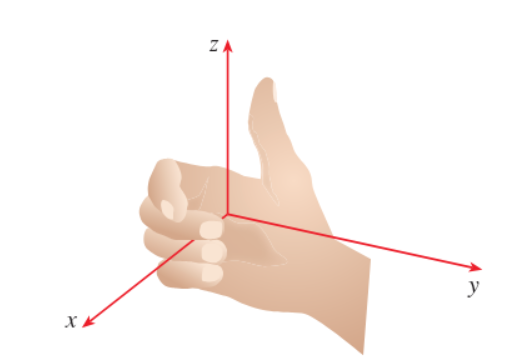
\includegraphics[width=0.5\textwidth]{images/right_hand_rule.png}
\end{center}

Projection of a point $(x, y, z)$ onto
\begin{itemize}
    \item $x-y$ axis: (x, y, 0)
    \item $x-z$ axis: (x, 0, z)
    \item $y-z$ axis: (0, y, z)
\end{itemize} 

\textbf{Distance formula in 3 dimensions:} Between two points $(x_1, y_1, z_1)$ and 
$(x_2, y_2. z_2)$, the distance is given by:
\[\sqrt{(x_2 - x_1)^2 + (y_2 - y_1)^2 +(z_2 - z_1)^2}\]

\textbf{Equation of a Sphere} with center at $(h, k, l)$ and radius $r$ is:

\[(x - h)^2 + (y - k)^2 + (z - l)^2 = r^2\]

\section{Vectors}

I will skip the basics, like vector addition definition, etc.

Components of a vector (for notation):
\[\aaa = \langle a_1, a_2, a_3 \rangle\]

Given points $A(x_1, y_1, z_1)$ and $B(x_2, y_2, z_2)$, 

\[\overrightarrow{AB} = \aaa = \langle x_2 - x_1, y_2 - y_1, z_2 - z_1 \rangle\]

\textbf{Magnitude of a vector} $\samplevec$ is 
\[|\aaa| = \sqrt{a_1^2 + a_2^2 + a_3^2}\]

\textbf{Unit vectors:} 
\[\ii = \langle 1, 0, 0 \rangle, \quad \jj = \langle 0, 1, 0 \rangle, \quad \kk = \langle 0, 0, 1 \rangle\]


\begin{tcolorbox}[colback=blue!5!white, colframe=blue!75!black, title=Algebraic Properties of Vectors in $\Rn$]
$\forall$ $\uu, \vv, \ww \in \Rn$ and scalars $c$ and $d$:
\begin{enumerate}
    \item \textbf{Commutativity of addition:} $\uu + \vv = \vv + \uu$
    \item \textbf{Associativity of addition:} $\uu + (\vv + \ww) = (\uu + \vv) + \ww$
    \item \textbf{Additive identity:} $\uu + \0 = \uu$
    \item \textbf{Additive inverse:} $\uu + (-\uu) = \0$
    \item \textbf{Distributivity of scalar multiplication over addition (vectors):} $c(\uu + \vv) = c\uu + c\vv$
    \item \textbf{Distributivity of scalar multiplication over addition (scalars):} $(c + d)\uu = c\uu + d\uu$
    \item \textbf{Associativity of scalar multiplication:} $(cd)\uu = c(d\uu)$
    \item \textbf{Scalar identity:} $1 \uu = \uu$
\end{enumerate}
\end{tcolorbox}

\section{The Dot Product}

\begin{definition}
If $\samplevec$ and $\bb = \langle b_1, b_2, b_3\rangle$ then the \textbf{dot product}
of $\aaa $ and $\bb$ is 
\[
\aaa \cdot \bb = a_1 b_1 + a_2 b_2 + a_3 b_3
\]
\end{definition}

\begin{tcolorbox}[colback=red!5!white, colframe=red!75!black, title=Properties of the Dot Product]
$\forall$ vectors $\aaa, \bb, \cc$ and scalar $c$:
\begin{enumerate}
    \item $\aaa \cdot \aaa = |\aaa|^2$
    \item $\aaa \cdot \bb = \bb \cdot \aaa$
    \item $\aaa \cdot (\bb + \cc) = \aaa \cdot \bb + \aaa \cdot \cc$
    \item $(c \aaa) \cdot \bb = c (\aaa \cdot \bb) = \aaa \cdot (c \bb)$
    \item $\0 \cdot \aaa = 0$
\end{enumerate}
\end{tcolorbox}

\begin{theorem}
    If $\theta$ is the angle between two vectors $\aaa, \bb$ then 
    \[\aaa \cdot \bb = |\aaa| |\bb| \cos \theta\]
\end{theorem}

\begin{corollary}
    Two vectors $\aaa, \bb$ are orthogonal iff $\aaa \cdot \bb = 0$
\end{corollary}

The \textbf{direction angles} of a non-zero vector $\aaa$ are the angles 
$\alpha, \beta, \gamma$ that $\aaa$ makes with the positive $x$-, $y$-, and $z$-axes, respectively.

The cosines of these angles are called \textbf{direction cosines}:

\[\cos \alpha = \frac{\aaa \cdot \ii}{|\aaa||\ii|} = \frac{a_1}{|\aaa|},
\quad \cos \beta = \frac{a_2}{|\aaa|},
\quad \cos \gamma = \frac{a_3}{|\aaa|}\]

Some nice properties of direction cosines:

\[\cos^2 \alpha + \cos^2 \beta + \cos^2 \gamma = 1\]

\[\frac{\aaa}{|\aaa|} = \langle \cos \alpha, \cos \beta, \cos \gamma \rangle\]

\textbf{Projections:}

The \textbf{projection of} $\bb$ \textbf{onto} $\aaa$ means we drop a perpendicular 
from the tip of $\bb$ onto the line spanned by $\aaa$. The resulting vector is called 
the vector projection of $\bb$ onto $\aaa$.

The \textbf{scalar projection of} $\bb$ \textbf{onto} $\aaa$ is the length of this 
projection, given by
\[
\text{comp}_{\aaa} \bb = |\bb|\cos\theta = \frac{\aaa \cdot \bb}{|\aaa|},
\]
where $\theta$ is the angle between $\aaa$ and $\bb$.

The \textbf{vector projection} of $\bb$ onto $\aaa$ is obtained by multiplying the 
unit vector in the direction of $\aaa$ by the scalar projection:
\[
\text{proj}_{\aaa} \bb = \left(\text{comp}_{\aaa} \bb \right)\frac{\aaa}{|\aaa|} 
= \frac{\aaa \cdot \bb}{|\aaa|^2}\aaa
\]

\section{The Cross Product}

\begin{definition}
For $\samplevec$ and $\bb = \langle b_1, b_2, b_3 \rangle$, the \textbf{cross product}
of $\aaa$ an $\bb$ is:
\[\aaa \times \bb = \langle a_2 b_3 - a_3 b_2, a_3 b_1 - a_1 b_3, a_1 b_2 - a_2 b_1 \rangle = \begin{vmatrix}
\mathbf{i} & \mathbf{j} & \mathbf{k} \\
a_1 & a_2 & a_3 \\
b_1 & b_2 & b_3
\end{vmatrix}
\]
\end{definition}

\begin{theorem}
    The vector $\aaa \times \bb$ is orthogonal to both $\aaa$ and $\bb$
\end{theorem}

\begin{theorem}
    The length of the cross product is given by: 
    \[ |\aaa \times \bb| = |\aaa| |\bb| \sin \theta\]
    where $\theta$is the angle between $\aaa$ and $\bb$.
\end{theorem}

\begin{corollary}
    Two nonzeros vectors $\aaa$ and $\bb$ are parallel iff 
    \[\aaa \times \bb = \0\]
\end{corollary}

\textbf{Area of parallelogram} determined by $\aaa$ and $\bb$ is $|\aaa \times \bb|$

\textbf{Area of parallelogram} determined by $\aaa$ and $\bb$ is $\frac{1}{2}|\aaa \times \bb|$

\textbf{IMPORTANT:} cross product is NOT commutative, and associate law for multiplication does not usually hold.

\begin{tcolorbox}[colback=red!5!white, colframe=red!75!black, title=Properties of the Cross Product]
$\forall$ vectors $\aaa, \bb, \cc$ and scalar $c$:
\begin{enumerate}
    \item $\aaa \times \bb = - \bb \times \aaa$
    \item $(c \aaa) \times \bb = c(\aaa \times \bb) = \aaa \times (c \bb)$
    \item $\aaa \times (\bb + \cc) = \aaa \times \bb + \aaa \times \cc$
    \item $(\aaa + \bb) \times \cc = \aaa \times \cc + \bb \times \cc$
    \item $\aaa \cdot (\bb \times \cc) = (\aaa \times \bb) \cdot \cc$
    \item $\aaa \times (\bb \times \cc) = (\aaa \cdot \cc) \bb - (\aaa \cdot \bb) \cc$
\end{enumerate}
\end{tcolorbox}

\textbf{Triple products:}

\[\aaa \cdot (\bb \times \cc) = \begin{vmatrix}
    a_1 & a_2 & a_3 \\
    b_1 & b_2 & b_3 \\
    c_1 & c_2 & c_3 \\
\end{vmatrix}\]


\textbf{Volume of the parallelipiped} determined by the vectors $\aaa, \bb$ and $\cc$
is:
\[V = |\aaa \cdot (\bb \times \cc)|\]

Useful: if the volume is 0, then the vectors must lie in the same plane, i.e. \textbf{coplanar}
\end{document}